%\documentclass{article}
%\usepackage{graphicx,subfigure}
%\begin{document}

\begin{figure}[!h]
  \centering
  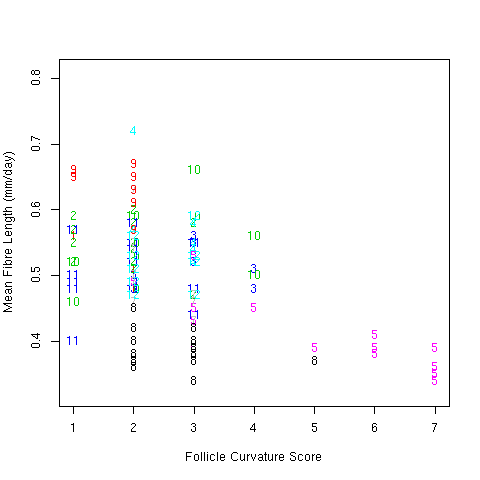
\includegraphics[width=1.0\textwidth]{fcfl.png}
  \caption{Plot of follicle curvature score against mean fibre length growth rate (mm/day). The numbered points reveal the Flock to which each data point belongs.The correlation of these points is -0.52 which is significant at the 1 percent level for 106 observations}
  \label{fig:fcfl}
\end{figure}

%\end{document}

